% Created 2021-03-14 Sun 16:03
% Intended LaTeX compiler: pdflatex
\documentclass[11pt]{article}
\usepackage[utf8]{inputenc}
\usepackage[T1]{fontenc}
\usepackage{graphicx}
\usepackage{grffile}
\usepackage{longtable}
\usepackage{wrapfig}
\usepackage{rotating}
\usepackage[normalem]{ulem}
\usepackage{amsmath}
\usepackage{textcomp}
\usepackage{amssymb}
\usepackage{capt-of}
\usepackage{hyperref}
\usepackage{xcolor}

\date{\today}
\title{Entropy in Evolutionary Algorithms}
\author{Lucas Blakeslee\footnote{\texttt{lqblakeslee@gmail.com}},
  Aengus McGuinness\footnote{\texttt{aengus82520@gmail.com}}}
\hypersetup{
 pdfauthor={},
 pdftitle={},
 pdfkeywords={},
 pdfsubject={},
 pdfcreator={Emacs 27.1 (Org mode 9.3)}, 
 pdflang={English}}

\begin{document}
\maketitle
%% \tableofcontents


\label{sec:org26f53e0}
\begin{abstract}
\label{sec:orga17da23}

Genetic algorithms (GAs) are an optimization technique inspired by
natural selection. GAs have yielded good results in certain practical
problems, yet there is still more to be understood about their
behavior on a theoretical level. One approach is to look at the
evolutionary process from the point of view of statistical mechanics,
and interpreting jumps in fitness as phase transitions. Toward this
goal we examine the behavior of \emph{entropy} in a GA that optimizes
a simple function.  We find that entropy increases as a new species
diversifies, but its upper bound decreases with most phase
transitions (which correspond to evolutionary steps).
\end{abstract}


%% -\textbf{- mode: org -}-


\section{Motivation}
\label{sec:org16abecd}
Genetic algorithms (GAs) are stochastic search algorithms based on the
process of natural evolution, solving for the 'fittest' solutions to a
problem. GAs are optimization algorithms, designed to maximize or
minimize certain functions. GAs are much more efficient than random or
exhaustive search algorithms (Kinnear, 1994), however, they do not
scale well with complexity (Radcliffe \& Surry, 1995). While specifics
may vary, there are some processes universal to GAs, which are:
population → fitness evaluation → selection → crossover → mutation,
repeat. Each organism in the population has its own 'chromosome,' or
set of characteristics. Here is where the resemblance to biological
evolution begins to weaken. The process continues to occur either
until some condition for termination has been met, or until a
pre-specified number of iterations has elapsed. Genetic algorithms
have been used in a variety of practical applications, from making
"evolved antennae" for spacecrafts and satellites to the estimation of
heat flux between sea ice and the atmosphere to predictive economic
models. Entropy and evolution have been often explored together, with
research on the subject going as far back as the 1870s, though
Schrödinger's 1944 book \emph{What is life?} sparked a wave of modern
interest. Here it was wondered how entropy would change over time in a
genetic algorithm, in order to attain a better theoretical grasp of
how they function.

\section{Hypothesis}
\label{sec:org26a3be1}
We hypothesized that entropy would gradually rise as small non-significant
mutations occured, and that occasionally one highly beneficial mutation in
an organism would cause entropy to rapidly decrease as that mutation was
selected for, as it spreads throughout the population, and then entropy would
begin to rise again, with the same cycle repeating. We hypothesized that the
upper bounds of the entropy would never reach levels they were previously at.


\section{Genetic algorithms in Brief}

In brief Genetic Algorithms attempt to find the maximum or minimum
value of a function, such as those shown in
Figure~\ref{fig:fit-func_pid3095791}

They do so by having a population of candidate values that take steps
through the domain of that function.  The steps have a random
component, but the randomness is directed by a principle akin to
natural selection: when a population member has a high fitness value,
it is more likely to survive and breed new population members that
share some of its characteristics.

Figure~\ref{fig:gen-info_pid3095791} shows an example of such an
evolution.

Some terminology is used in talking about GA evolution:

\begin{description}
\item[population] The collection of values currently being considered
  as possible solutions to the problem.
\item[fitness] A function 
\end{description}


\begin{figure}
  \label{fig:fit-func_pid3095791}
  \centering
  \resizebox{0.7\linewidth}{!}{%
  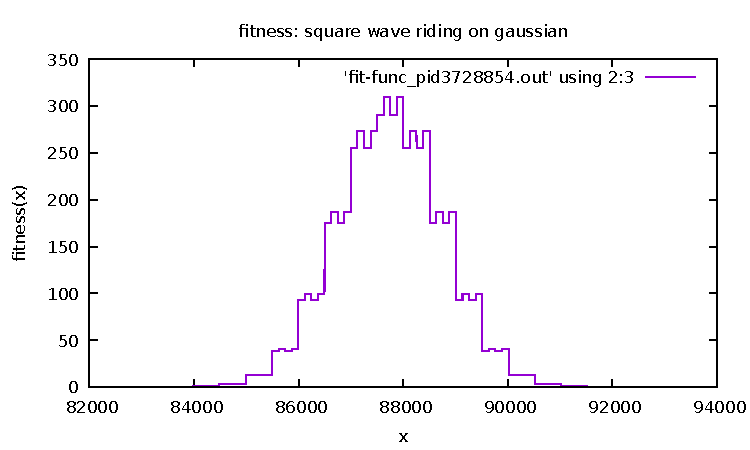
\includegraphics{fit-func_pid3728854.pdf}
  }
  \caption{One example of a fitness function.}
  \label{fig:multi-step}
\end{figure}


\section{Approach}
\label{sec:org8c588e5}

To explore how the entropy of the GA population behaves we crafted an
optimization problem that would bring out some well defined
steps in fitness improvement and also allow a period of statis between 





\section{Methods}
\label{sec:org2c55902}
Originally, we constructed a genetic algorithm to find the maxima of a
polynomial using the IEEE 754 floating point standard to represent the
chromosomes of an inidividual. The polynomial was structured as: ax\textsuperscript{7}
+ ax\textsuperscript{6} \ldots + ax\textsuperscript{2} + ax + a. Later we
decided to have the software find the maxima of other types of functions,
in our case a $\sin$ wave riding on top of a gaussian. $ P(x) = \frac{1}{{\sigma \sqrt {2\pi } }} e^{{{ - \left( {x - \mu} \right)^2 } \mathord{\left/ {\vphantom {{ - \left( {x - \mu } \right)^2 } {2\sigma ^2 }}} \right. \kern-\nulldelimiterspace} {2\sigma ^2 }}} $
\color{red} \textbf{!! We need to include a plot of this !!}
\color{black}

The population of 10,000 underwent the standard evalutation, selection,
crossover, and mutation of a  GA, with information about the population
being collected at the end of each iteration. Diversity was measured using
the hamming distance between the binary strings of two organisms, and the
Shannon entropy of the population was calculated at the end of each generation.
Additionally, the elite and average fitnesses of the population were tracked.

\subsection{Mate Drift vs Bitflip}
Originally we represented individuals with a 32 bit binary string, and occasionally 
flipped a random bit as mutation. Depending on whether a bit in the sign, the mantissa, 
or the exponent was flipped, the impact the mutation had could vary drastically,
much like how in biological evolution many mutations are silent or have little impact,
 however occasionally  they can lead to very rapid change. Using this technique,
 we had a very clear understanding of what mutation actually is. However, we found 
that this led to some unprecedented issues regarding the numerical limitations
of a 32 bit string. For example, in the string $0 01111111 11111111111111111111111$,
the probability of the first bits flipping to a 1and remaining advantageous is incredibly
low, as the majority of the other bits would have to flip to a 0.

\section{Results}
\label{sec:orged0917a}
We found that rapid drops in entropy accompanied increases of fitness, and
additionally that the upper bound of the entropy did not get as high
as it was at previous levels.


\begin{figure}
  \label{fig:gen-info_pid3095791}
  \centering
  \resizebox{0.5\linewidth}{!}{%
    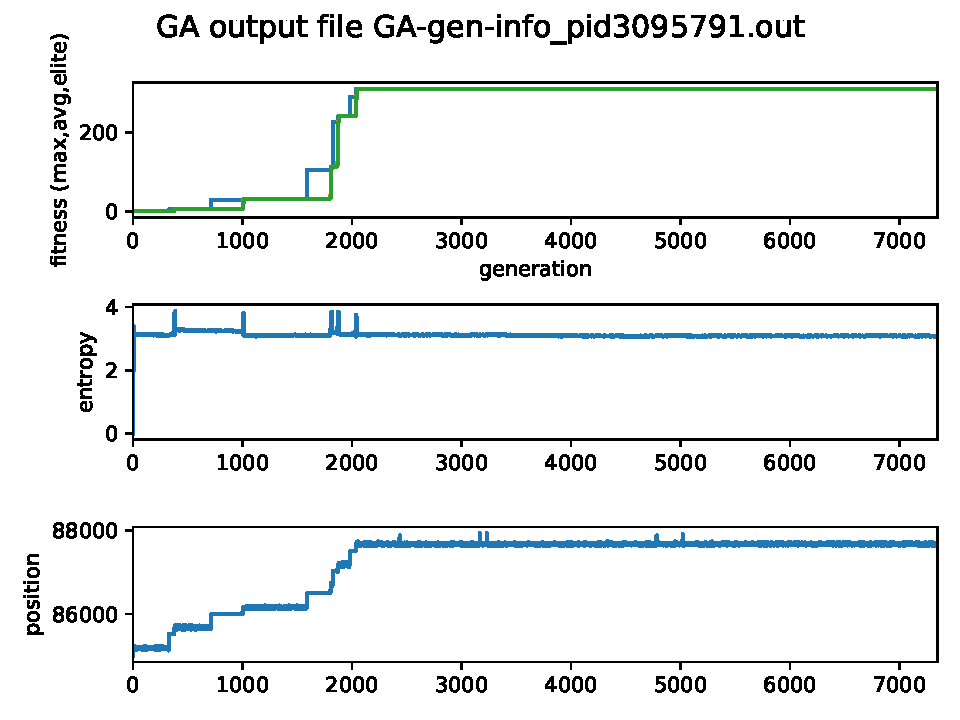
\includegraphics{GA-gen-info_pid3095791.out.pdf}
  }
  \caption{One example of evolution.}
  \label{fig:multi-step}
\end{figure}

\begin{figure}
\end{figure}

\section{Discussion}
\label{sec:org7999995}
\subsection{what does this mean?}
\label{sec:orgf7b36ed}
content...

\subsection{Limitations to genetic algorithms}
\label{sec:org148bf83}
There are some limitations to genetic algorithms. For example, one must
have a very clear understanding of the problem, constraints, the data
structure, etc. Additionally, genetic algorithms do not scale well with
complexity -- problems with large numbers of elements often become exponentially
more difficult to compute. There is also the difficulty of ensuring the
algorithm doesn't get stuck on a local maxima rather than the global one.

\subsection{Future work}
\label{sec:org0f04af1}
Going forwards, it could be interesting to optimize a genetic algorithm from the standpoint of its entropy.

\section{References}
\label{sec:org9dc046e}
\textbf{these will ultimately need to be alphebatized by last name of the first author} \textbf{the citation style should be consistent, I was thinking APA}

Kinnear, K. E. (1994). In K. E. Kinnear (Ed.), \emph{Advances in Genetic Programming} (pp. 3-17). Cambridge: MIT Press.

Radcliffe N.J., Surry P.D. (1995) Fundamental limitations on search algorithms: Evolutionary computing in perspective.
In: van Leeuwen J. (eds) Computer Science Today. Lecture Notes in Computer Science, vol 1000. Springer, Berlin, Heidelberg.
\url{https://doi.org/10.1007/BFb0015249}
\end{document}
